\section{Hagan Rowlenstino/1174040}
	\subsection{Soal 1}
	library matplotlib adalah sebuah library untuk memplotting 2 Dimensi yang output nya adalah gambar publikasi yang bermutu di banyak format hardocpy serta lingkungan interaktif berbagai platform

	\subsection{Soal 2}
	untuk membuat sumbu x dan y :
	\lstinputlisting{src/6/1174040/Teori/chap6_1174040_2.py}

	\subsection{Soal 3}
	\begin{itemize}
		\item PLot Garis :

		\lstinputlisting[firstline=8, lastline=13]{src/6/1174040/Teori/chap6_1174040_3.py}

		\item Plot Sebaran

		\lstinputlisting[firstline=15, lastline=18]{src/6/1174040/Teori/chap6_1174040_3.py}

		\item Plot Batang / Histogram

		\lstinputlisting[firstline=20, lastline=23]{src/6/1174040/Teori/chap6_1174040_3.py}

		\item Pie

		\lstinputlisting[firstline=26, lastline=35]{src/6/1174040/Teori/chap6_1174040_3.py}

	\end{itemize}

	\subsection{Soal 4}
	\begin{itemize}
		\item Legend : Penjelasan garis beserta contoh dari garis yang dijelaskan tersebut. untuk membuat legend dapat menggunakan sintaks berikut :

		\begin{verbatim} legend('legend grafik1',…,'legend grafikN','Nilai Pos') \end{verbatim}
		
		\item Label : Memberikan penamaan untuk skala(sumbu) yang kita buat. untuk menambahkan label, kita dapat menggunakan sintaks berikut :

		\begin{verbatim} 
		xlabel(‘teks horizontal axis’)

		ylabel(‘teks vertikal axis’)
		\end{verbatim}
	\end{itemize}

	\subsection {Soal 5}
	Subplot pada matplotlib berfungsi untuk membuat banyak plot grafik dalam satu figure saja.
	dimana  subplot dapat kita definisikan sebagai berikut :
	
	\begin{verbatim} subplot(m,n,i) 
	\end{verbatim}
	Dimana m adalah tinggi nya, n adalah lebar nya dan i adalah urutan penempatannya.
	Untuk membuat 9 subplot dapat dilihati dari contoh dibawah ini :

	\lstinputlisting{src/6/1174040/Teori/chap6_1174040_5.py}

	\begin{figure}[ht]
            \centerline{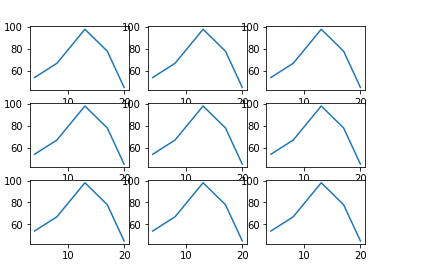
\includegraphics[width=0.5\textwidth]{figures/6/1174040/Teori/1174040_no5.png}}
            \caption{No. 5}
            \label{1174040_chap6_no5}
            \end{figure}

	\subsection{Soal 6}
	color yang dapat digunakan adalah red(r),blue(b),green(g),cyan(c),magenta(m),yellow(y),black(k),white(w)

	\subsection{Soal 7}
	fungsi Hist digunakan untuk membuat histogram yang berfungsi untuk menampilkan frekuensi data dengan menggunakan grafik batang

	\lstinputlisting{src/6/1174040/Teori/chap6_1174040_hist.py}

	\begin{figure}[ht]
            \centerline{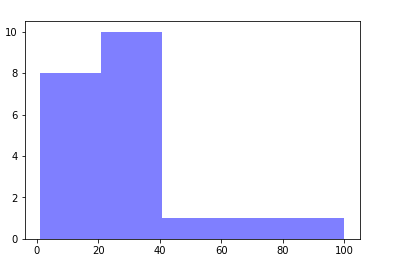
\includegraphics[width=0.5\textwidth]{figures/6/1174040/Teori/1174040_no7.png}}
            \caption{No. 7}
            \label{1174040_chap6_no7}
            \end{figure}

	\subsection{Soal 8}
	\begin{itemize}
		\item Labels : Untuk memberi penamaan terhadap setiap potongan dari pie
		\item colors : Untuk memberikan warna spesifik terhadap potongan potongan pie, jika tidak diberi warna maka dia akan menggambi warna dari pie yang telah berjalan
		\item startangle : Untuk menetapkan dari sudut mana grafik tersebut akan dimulai
		\item shadow : untuk memberikan efek bayangan di bawah pie maupun potongannya
		\item explode : untuk menentukan seerapa jauh pemisahkan potongan pie dari potongan - potongan lainnya
		\item autopct : untuk memberikan nilai atau skalal numeric pada label didalam potongan pie . seperti mengubah dari 10 menjadi 10.0
	\end{itemize}

	\subsection{Cek Plagiarisme}
	
	\begin{figure}[ht]
            \centerline{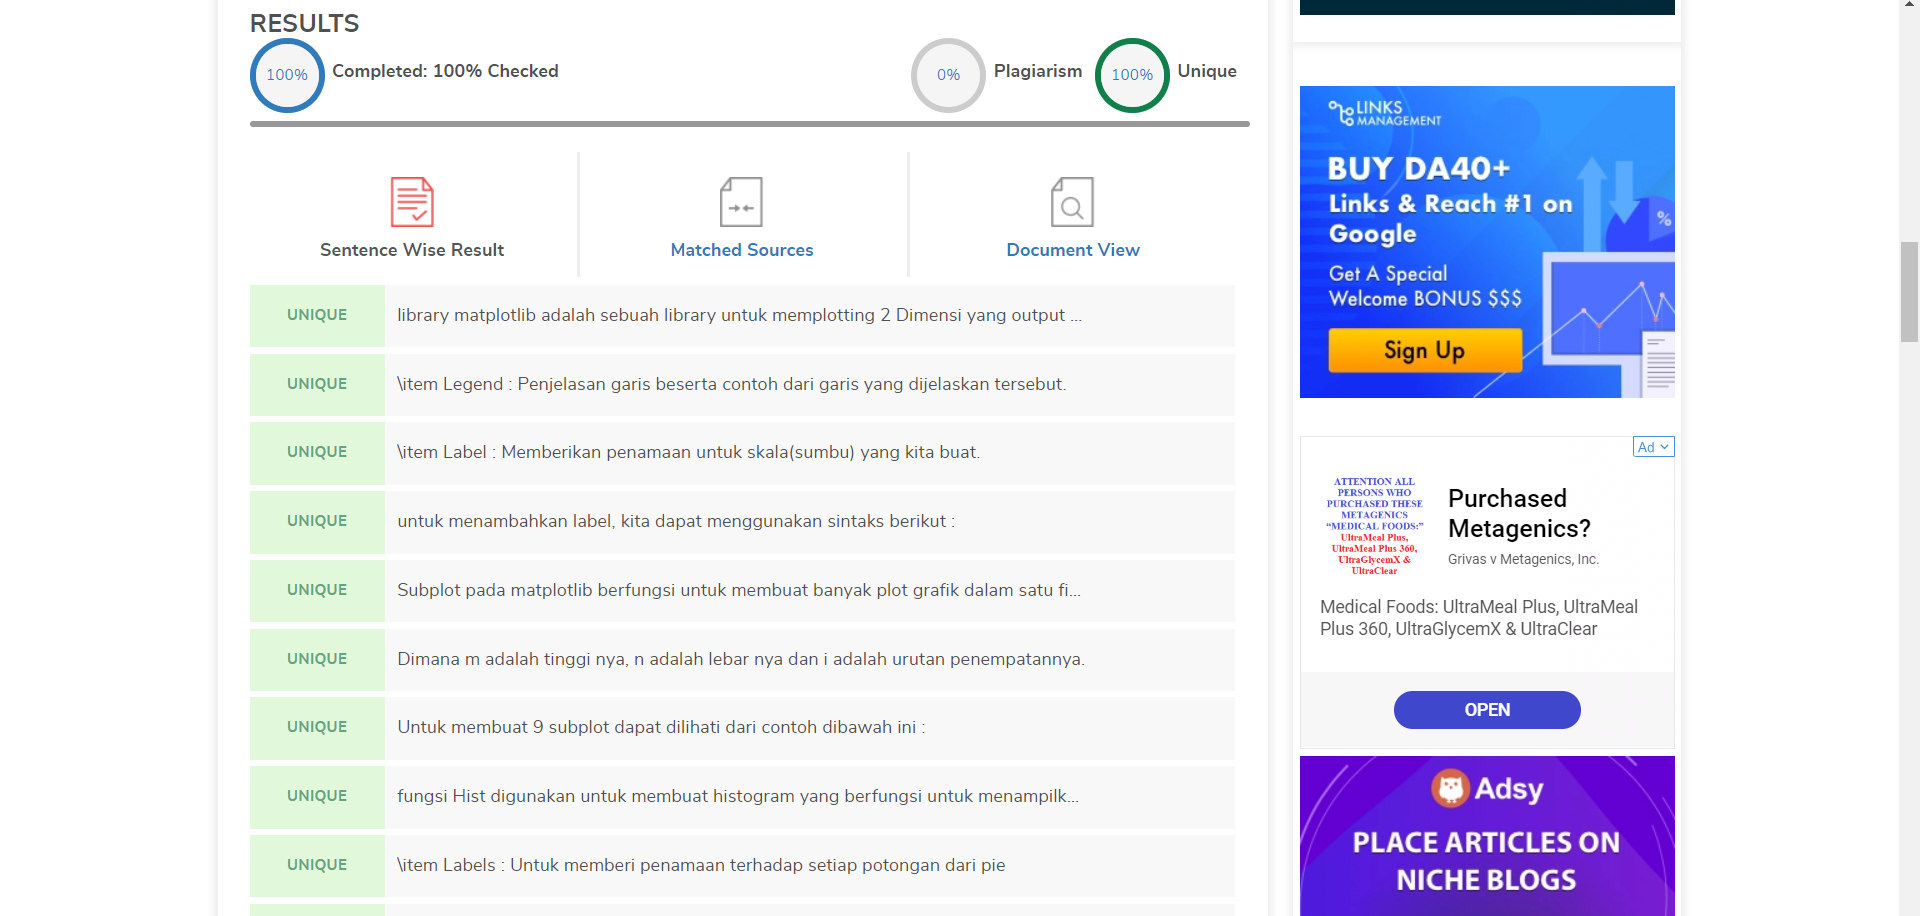
\includegraphics[width=0.5\textwidth]{figures/6/1174040/Teori/1174040_plagiat.png}}
            \caption{Cek Plagiarisme}
            \label{1174040_chap6_plagiat}
            \end{figure}
			
\section{Irvan Rizkiansyah/1174043}
	\subsection{Nomor 1}
		matplotlib merupakan library plotting 2D Python dan berfungsi untuk membuat plot, histogram, grafik batang, scatterplot, dan masih banyak yang lainnya hanya dengan beberapa baris code saja.
		
	\subsection{Nomor 2}
	Pembuatan sumbu X dan Y di matplotlib, mirip dengan membuat sebuah variabel yang mempunyai array. Kemudian variabel yang dibuat yang nanti-nya akan menjadi sumbu X dan Y dan akan dipanggil menggunakan fungsi plot.
		\lstinputlisting[firstline=8, lastline=14]{src/6/1174043/Teori/chap6_1174043_no2.py}
	
	\subsection{Nomor 3}
	Perbedaan fungsi yang ada pada matplotlib :
		\begin{itemize}
			\item Fungsi scatter atau plot sebaran merupakan sebuah grafik yang menunjukkan hubungan dari dua set data, seperti halnya hubungan dari tinggi badan dan berat badan.
			Cara menggunakannya dengan memanggil fungsi scatter yang terdapat pada matplotlib \begin{verbatim} matplotlib.pyplot.scatter(x,y) \end{verbatim}
			
			\item Fungsi histogram merupakan sebuah grafik yang akan menampilkan frekuensi data menggunakan sebuah batang.
			Cara menggunakannya dengan memanggil fungsi hist yang terdapat pada matplotlb \begin{verbatim} matplotlib.pyplot.hist(x,y) \end{verbatim}
			
			\item Fungsi plot garis atau plot sinus merupakan sebuah grafik yang menunjukkan frekuensi data menggunakan garis.
			Cara menggunakannya dengan memanggil fungsi plot yang terdapat pada matplotlib \begin{verbatim} matplotlib.pyplot.plot(x,y) \end{verbatim}
			
		\end{itemize}
	Dan masih banyak yang lainnya.
	\subsection{Nomor 4}
	Fungsi legend merupakan dimana akan menamai sebuah bar pada grafik untuk membedakan bar tersebut dengan bar yang lainnya, dimana jika terdapat banyak bar pada grafik tersebut. Sedangkan fungsi label untuk menamai sumbu x dan sumbu y.
	Cara menggunakannya hanya tinggal memanggil fungsi legend dan fungsi label yang terdapat pada matplotlib dan memberikan nama untuk legend dan label tersebut. Contohnya :
		\lstinputlisting[firstline=8, lastline=19]{src/6/1174043/Teori/chap6_1174043_legend.py}
	
	\subsection{Nomor 5}
	Fungsi subplot adalah untuk memanggil banyak grafik hanyak dengan sekali panggil saja. Cara kerja dari fungsi subplot ini sendiri cukup simpel, dimana cukup memanggil fungsi subplot yang terdapat pada matplotlib 
	\begin{verbatim} matplotlib.pyplot.subplot(nbaris, nkolom, index) \end{verbatim}
	Dibawah ini merupakan ilustrasi dan parameter apa saja yang digunakan jika ingin menggambar plot dengan 9 sub plot :
		\lstinputlisting[firstline=8, lastline=54]{src/6/1174043/Teori/chap6_1174043_subplot.py}
		
	\subsection{Nomor 6}
	Matplotlib mengenal beberapa format untuk color diantaranya :
		\begin{itemize}
			\item RGB atau RGBA contohnya (0.1, 0.2, 0.5)
			\item hex RGB atau RGBA contohnya '\#0F0F0F
			\item Representasi string dari nilai float contohnya '0.5'
			\item atau hanya seperti kata awal dari warna tersebut yang ingin digunakan contohnya warna Cyan maka hanya perlu menggunakan 'c', warna Green maka hanya perlu menggunakan 'g' dan masih banyak yang lainnya seperti 'b', 'r', 'm', dan yang lainnya
			\item X11/CSS4 nama warna
			\item nama dari xkcd color survey contohnya 'xkcd:sky blue'
			\item Tableau Color dari 'T10' pallette kategorikal contohnya 'tab:olive'
			
		\end{itemize}
	
	\subsection{Nomor 7}
	Fungsi hist merupakan fungsi untuk menggunakan grafik bar atau batang, dimana frekuensi setiap elemen data yang ada pada daftar ditunjukkan dengan grafik histogram. Angka yang dikelompokkan dalam bentuk rentang tertentu yang sudah di tentukan dsebut bins.
		\lstinputlisting[firstline=8, lastline=12]{src/6/1174043/Teori/chap6_1174043_histogram.py}
	
	\subsection{Nomor 8}
	Parameter yang terdapat pada fungsi pie :
		\begin{itemize}
			\item labels : dimana berfungsi untuk memberi nama untuk setiap slice yang terdapat pada grafik pie
			\item colors : dimana berfungsi untuk memberikan warna untuk setiap slice yang terdapat pada gradik pie
			\item startangle : dimana berfungsi jika tidak tidak ada, maka awalan putaran dari grafik pie berlawanan dari arah jarum jam dari titik sumbu x
			\item shadow : dimana berfungsi untuk memberikan efek grafis bayangan pada grafik pie
			\item explode : dimana berfungsi untuk menentukan fraksi dari jari-jari untuk mengimbangi setiap slice menggunakan sumbu x
			\item autopct : string atau fungsi yang digunakan untuk label pada slice dengan nilai numerik, maka label akan ditempatkan didalam slice.			
		\end{itemize}
	